\chapter{Expermients and Results}

\section{Introduction}

This section describes the experiments and methodology used to evaluate the proposed solutions. 
The experiments were conducted on two different datasets: BrightKite and CitiBike, which are 
real-world datasets, and we included a synthetic dataset for parameter tuning.

\section{Datasets}

\subsection{BrightKite Data}

\subsubsection{Overview}

BrightKite was a location-based social network where users shared their locations by checking in at 
different places.

The dataset contains check-ins from users, and each check-in contains the user's ID, the location's ID, 
the timestamp, and the location's geographical coordinates.

BrightKite data was used by Thodoris Lykouris and Sergei Vassilvitskii in their paper "Competitive 
Caching with Machine Learned Advice" \cite{datasets-reference} and the dataset is publicly available
at \cite{brightkite-data}.

From this dataset, we created multiple instances of the caching problem, by considering each user 
as a tenant for our multi-tenant caching problem, location IDs as items or pages to be cached, and 
check-ins as item or page accesses. 

\subsubsection{Processing}

Similar to the work done by Thodoris Lykouris and Sergei Vassilvitskii in \cite{datasets-reference},
we selected the top users where the optimal cache algorithm (Belady's or clairvoyant) had more cache 
faults, to select the most challenging users from the dataset.

Then we created 6 instances of the multi-tenant caching problem, by considering each of the most 
challenging users as a tenant, the locations as items to be cached, and the check-ins as item accesses.

We took 36 most challenging users from the dataset, and created 6 instances of the multi-tenant caching
problem, two of them with 4 tenants, two with 5 tenants, one with 8 tenants, and one with 10 tenants.

Information of the selected users, with number of accesses, number of unique items, and number of cache
faults for the optimal cache algorithm (with cache size equal to 50), rank and user ID, is shown in
Appendix \ref{appendix:brightike-top-36-users}.

The number of accesses per user is from 1300 to 2100, with most of them having 2100. The number of
unique items per user is from 300 to 1300, with many of them having around 600. The number of cache
faults for the optimal cache algorithm is from 10 to 164, with most of them having around 20 or 30.

The cache size recommendations for each tenant started at 40 and kept increasing by 10 until 
the number of extra cache faults for the optimal cache algorithm using a buffer size of the 
recommendation was less than 40.

The number of extra cache faults is the number of cache faults minus the number of unique items accessed, 
since the first access of each item is always a cache fault.

\subsection{CitiBike Data}

\subsubsection{Overview}

CitiBike is a popular bike-sharing service in New York City. We consider citibike trip histories, 
in which each ride is a cache item access. Experiments were made with monthly data from 2023, 
the dataset is publicly available at \cite{citibike-data}.

The dataset contains information about each trip, the start and end station IDs, if the bike
was electric or classic, if the rider is a member or a casual rider, 
the start date and time that was used to sort the data, and more information not used in the 
experiments.

CitiBike data was also used by Thodoris Lykouris and Sergei Vassilvitskii in their paper "Competitive 
Caching with Machine Learned Advice" \cite{datasets-reference}.

We made artificial tenants by considering if the bike was electric or classic, and if the rider 
was a member or a casual rider, therefore we have 4 tenants: electric members, electric casuals,
classic members, and classic casuals.

\subsubsection{Processing}

We made three experiments: 

\begin{itemize}
    \item In the first one, we considered the pair (start\_station\_id, end\_station\_id) to be 
    the items to be cached, so that two trips are only considered the same if they have the 
    same start and end stations.
    \item In the second one, we numbered start stations from 1 to the number of unique start 
    stations, and end stations from 1 to the number of unique end stations, and then considered 
    the pair \(\left(\lfloor \frac{\text{start\_station\_rank}}{5} \rfloor, \lfloor \frac{\text{end\_station\_rank}}{5} \rfloor\right)\) 
    to be the items to be cached.
    \item In the third one, we considered the start station ID to be the item to be cached.
\end{itemize}

The number of unique items and number of accesses in each experiment is shown on the following tables.

\begin{table}[ht]
    \centering
    \small
    \caption{Summary per tenant in the CitiBike experiment 1.}
    \csvautotabular{data/citibike_exp_1_case_2_summary.csv}
    \label{tab:citibike-exp-1-case-2-summary}
\end{table}

\begin{table}[ht]
    \centering
    \small
    \caption{Summary per tenant in the CitiBike experiment 2.}
    \csvautotabular{data/citibike_exp_2_case_3_summary.csv}
    \label{tab:citibike-exp-2-case-3-summary}
\end{table}

\begin{table}[ht]
    \centering
    \small
    \caption{Summary per tenant in the CitiBike experiment 3.}
    \csvautotabular{data/citibike_exp_3_case_4_summary.csv}
    \label{tab:citibike-exp-3-case-4-summary}
\end{table}

% \newpage

The cache size recommendations for each tenant started at 5000, 2000, and 50 in the first, 
second, and third experiments, respectively, and kept increasing by 1000, 400, and 10 until 
the extra cache fault ratio for the optimal cache algorithm using a buffer size of the 
recommendation was less than 20\%, 10\%, and 5\%, respectively.

The extra cache fault ratio is the number of extra cache faults divided by the number of extra 
accesses, where the number of extra cache faults is the number of cache faults minus the number 
of unique items accessed, and the number of extra accesses is the number of accesses minus the 
number of unique items accessed.

\subsection{Random Data}

\subsubsection{Overview}

Random data was used for hyperparameter tuning, testing, and validation of the algorithms, 
but not in the experiments.

It has been shown that when the probability distribution of the data access pattern is constant 
over time, LFU yields the highest performance \cite{lfu-highest-perf-zipf} 
\cite{lfu-highest-perf-inproc} \cite{tiny-lfu}. Therefore, we did not generate data using only 
one probability distribution, as this would favor LFU and not take into account the problem of 
changing access patterns over time.

\subsubsection{Generation}

To generate random data, we used the following probability distributions:

\begin{itemize}
    \item Zipfian distribution, since a popular assumption is that cache workloads follow it 
    \cite{zipf-dist-cache-1} \cite{zipf-dist-cache-2} \cite{zipf-dist-cache-3} 
    \cite{lfu-highest-perf-zipf}.
    \item Pareto distribution, since it has been shown that storage and internet traffic traces 
    are well modeled by it \cite{pareto-dist-workload} \cite{pareto-dist-workload-2} 
    \cite{pareto-dist-workload-3}.
    \item Normal distribution; we used it less than the other distributions since it is not 
    commonly used in cache workloads, but it was used in \cite{memory-aware-buffer-pool-manager}.
    \item Uniform distribution; we used it less than the other distributions since it is not 
    commonly used in cache workloads, but it was used in \cite{memory-aware-buffer-pool-manager}.
\end{itemize}

To address the problem of changing access patterns over time, in some cases, we generated data 
using one distribution for a period of time, and then changed the distribution to another one. 
In many cases, the distribution was the same, but we renumbered the most accessed items.

To address the problem of correlated accesses, in some cases, when generating data for the 
tenants, we generated correlated accesses to some items, causing them to be accessed together 
during certain periods of time.

To handle multi tenancy, in some cases we randomly merged the data of the tenants, and in 
other cases we splitted the data of each tenant into chunks, and then randomly merged the
chunks.

\section{Testing and Validation}

\subsection{Data Validation}

In order to ensure the integrity of the data, we validated each case for the experiments and 
the randomly generated data.

For each case, we checked that each tenant had the correct number of accesses and the correct 
number of unique items, both by script and by visually plotting the data to ensure it was 
correctly generated.

Additional integrity checks related to buffer sizes, priority levels, and tenant information 
were also performed.

\subsection{Algorithm Validation}

In order to validate the algorithms, we simulated the cache eviction process for each case, 
keeping track of the cache state and the cache faults, and performing integrity checks related 
to the cache state, cache hits, and faults.

Checks related to the tenant selection policy were performed to ensure that each tenant had at 
least the minimum buffer size promised at any time, did not exceed the maximum buffer size 
promised at any time, and was selected according to the tenant selection policy.

Additional checks related to the cache eviction policy were performed to ensure that the 
eviction policy was correctly implemented and worked as expected.

\section{Experiments}

\subsection{Overview}

For each experiment type, we ran each cache eviction policy, using the fault ratio with 
cache used tenant selection policy on the following datasets:

\begin{itemize}
    \item BrightKite experiment data.
    \item CitiBike 1st experiment data.
    \item CitiBike 2nd experiment data.
    \item CitiBike 3rd experiment data.
\end{itemize}

The minimum buffer size per tenant was set to 40\% of the cache size recommendation, and the
maximum buffer size per tenant was set to 250\% of the cache size recommendation for the 
BrightKite experiment, and 220\% of the cache size recommendation for the CitiBike experiments.

The total buffer size was set to 80\% of the sum of the cache size recommendations for each 
tenant.

\subsection{Hit Ratio Per Cache Size Experiment}

In the hit ratio per cache size experiment, we ran the cache eviction policies with 10 different
cache sizes, and computed the hit ratio for each cache size and tenant.

The cache sizes used per experiment were:

\begin{itemize}
    \item BrightKite experiment: 50, 75, 100, 125, 150, 175, 200, 225, 250, 275.
    \item CitiBike 1st experiment: 4000, 8000, 12000, 16000, 20000, 24000, 28000, 32000, 36000, 40000.
    \item CitiBike 2nd experiment: 3000, 6000, 9000, 12000, 15000, 18000, 21000, 24000, 27000, 30000.
    \item CitiBike 3rd experiment: 200, 400, 600, 800, 1000, 1200, 1400, 1600, 1800, 2000.
\end{itemize}

These sizes were selected based on the number of unique items and the number of accesses, as 
well as the number of cache faults for the optimal cache algorithm.

The cache size recommendations for each tenant were scaled based on the total buffer size to 
keep the total buffer size at 80\% of the sum of the cache size recommendations for each tenant.

Minimum and maximum buffer sizes were also scaled based on the cache size recommendations.

All tenant priorities were equal in this experiment.

\subsubsection*{Results in BrightKite Dataset}

The hit ratio per cache size per tenant for the BrightKite dataset is shown in Figure 
\ref{fig:hit_ratio_per_cache_size_exp_brightkite}.

The penalty function score (fault score) per cache size for the BrightKite dataset 
is shown in Table \ref{tab:fault-score-per-buffer-size-brightkite}.

By comparing LRU with Fault Ratio with Cache Used Policy (LRU in Figure and Table) with LRU 
using Naive Policy (NaiveLRU in Figure and Table), we observe that the Fault Ratio with Cache 
Used Policy improves with a higher cache size, performing similarly or worse with smaller cache 
sizes, but better with larger cache sizes, outperforming the NaiveLRU policy for all tenants 
after a cache size of 125.

We observe that most of the cache eviction policies perform well with the Fault Ratio with 
Cache Used Policy, many of them outperforming separate or naive LRU policies with a 20\% 
higher cache size (since they show a 0 penalty score) for different cache sizes.

LRU-2, LIRS, and MQ perform particularly well, showing a 0 penalty score for all cache sizes of 
125 or higher and high hit ratios for all tenants. LIRS results are particularly interesting 
since it is a low-overhead policy, and LRU-2 is performing very well.

\begin{figure}[H]
    \centering
    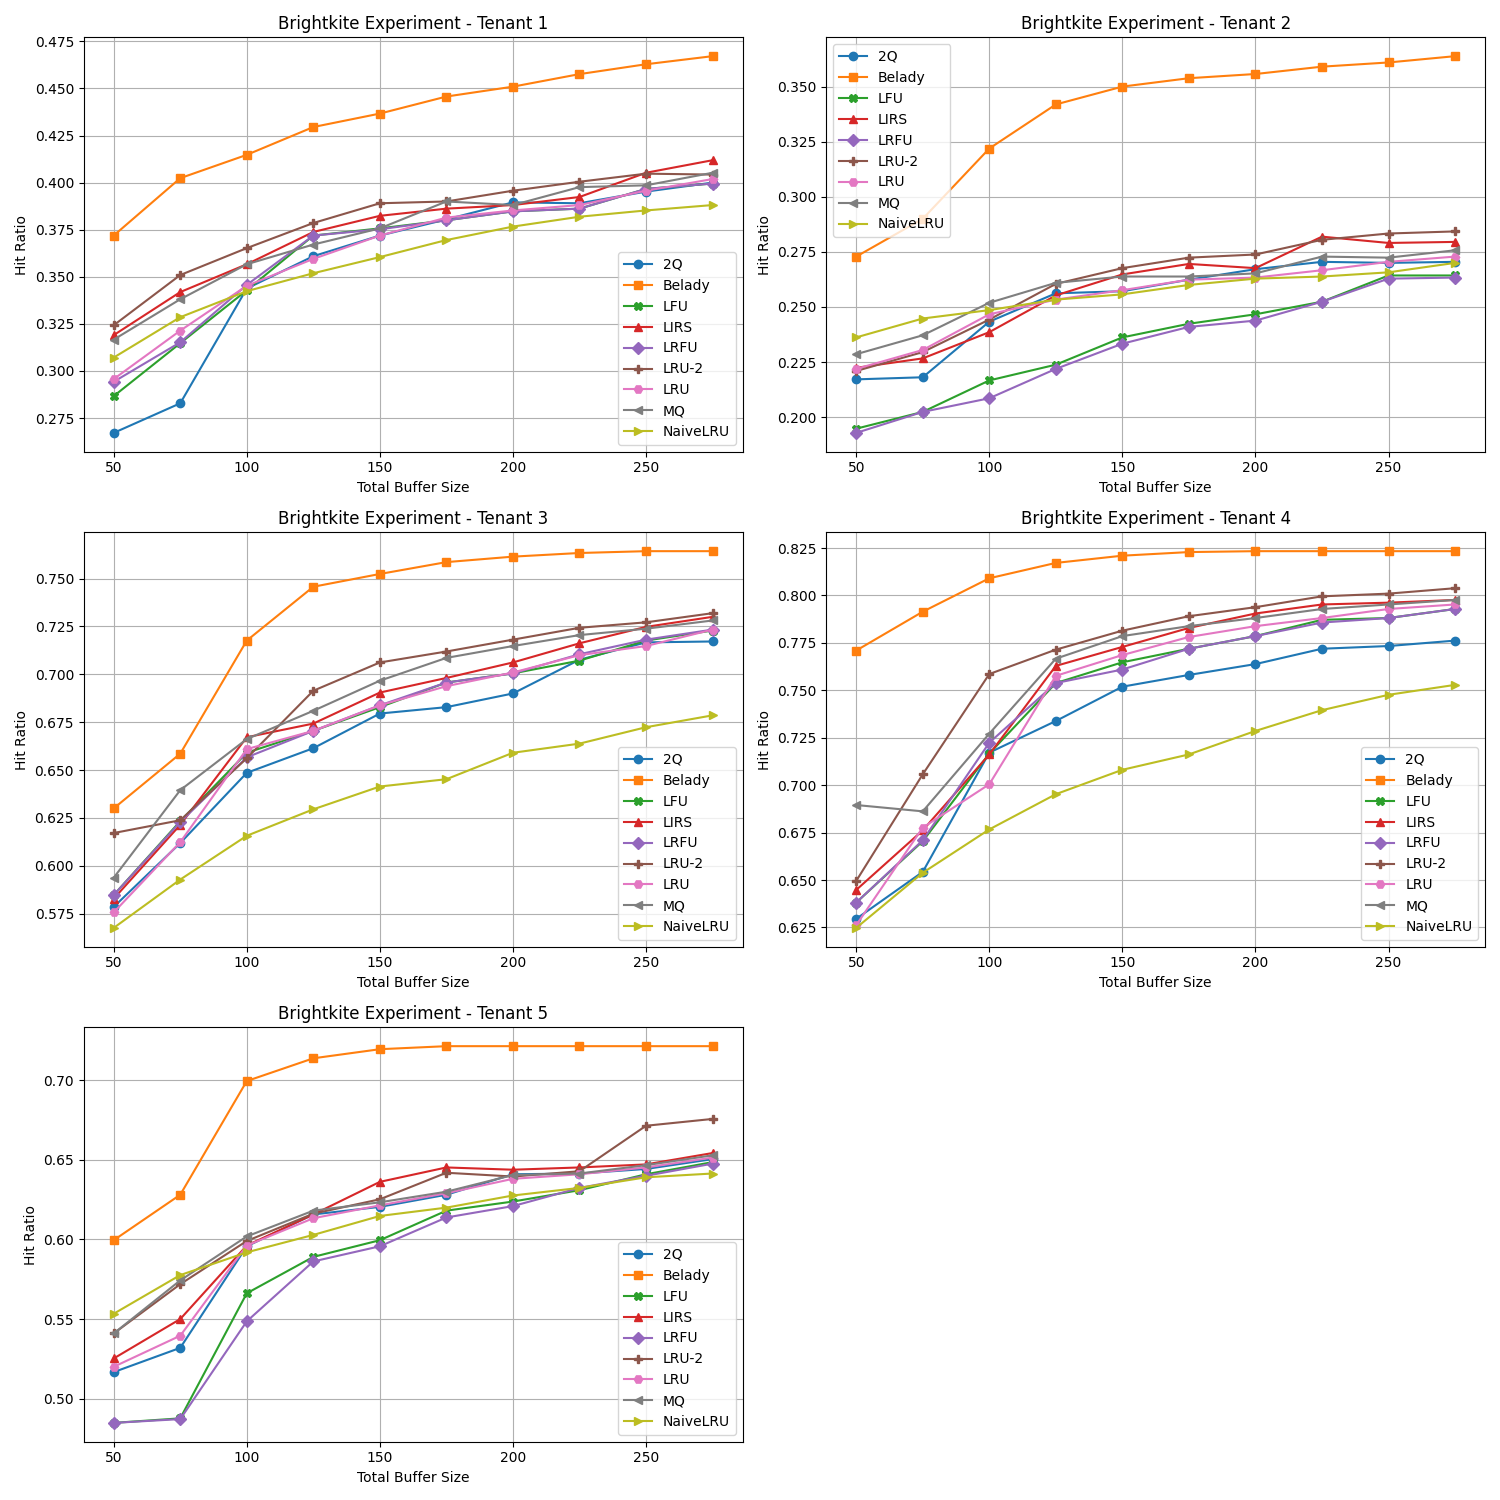
\includegraphics[width=0.75\textwidth]{hit_ratio_per_cache_size_exp_brightkite.png}
    \caption{Hit ratio per cache size per tenant for the BrightKite dataset}
    \label{fig:hit_ratio_per_cache_size_exp_brightkite}
\end{figure}

\begin{table}[H]
    \centering
    \small
    \caption{Penalty function score (fault score) per cache size for the BrightKite dataset}
    \csvautotabular{data/fault_score_per_buffer_size_brightkite.csv}
    \label{tab:fault-score-per-buffer-size-brightkite}
\end{table}

\subsubsection*{Results in CitiBike Dataset}

The hit ratio per cache size per tenant for the first experiment with the CitiBike dataset is
shown in Figure \ref{fig:hit_ratio_per_cache_size_exp_citibike}.

The penalty function score (fault score) per cache size for the first, second and third 
experiments with the CitiBike dataset are shown in Tables 
\ref{tab:fault-score-per-buffer-size-citibike}, \ref{tab:fault-score-per-buffer-size-citibike-2}
and \ref{tab:fault-score-per-buffer-size-citibike-3} respectively.

In the first experiment, we observe that most of the cache eviction policies perform very 
well with the Fault Ratio with Cache Used Policy, many of them outperforming separate or 
naive LRU  policies with a 20\% higher cache size (since they show a 0 penalty score) for 
different cache sizes.

In other experiments, results are not as good as in the first experiment, still showing
good results and low penalty scores with several cache eviction policies.

LFU, LRU-2, LIRS, and MQ perform particularly well, showing a 0 penalty score for most cache 
sizes. LIRS results are particularly interesting since it is a low-overhead policy, 
and LFU is performing very well. 

Note that even though LFU is performing very well in this dataset, it is not practical in some 
real-world scenarios since it suffers greatly from access pattern changes.

\begin{figure}[H]
    \centering
    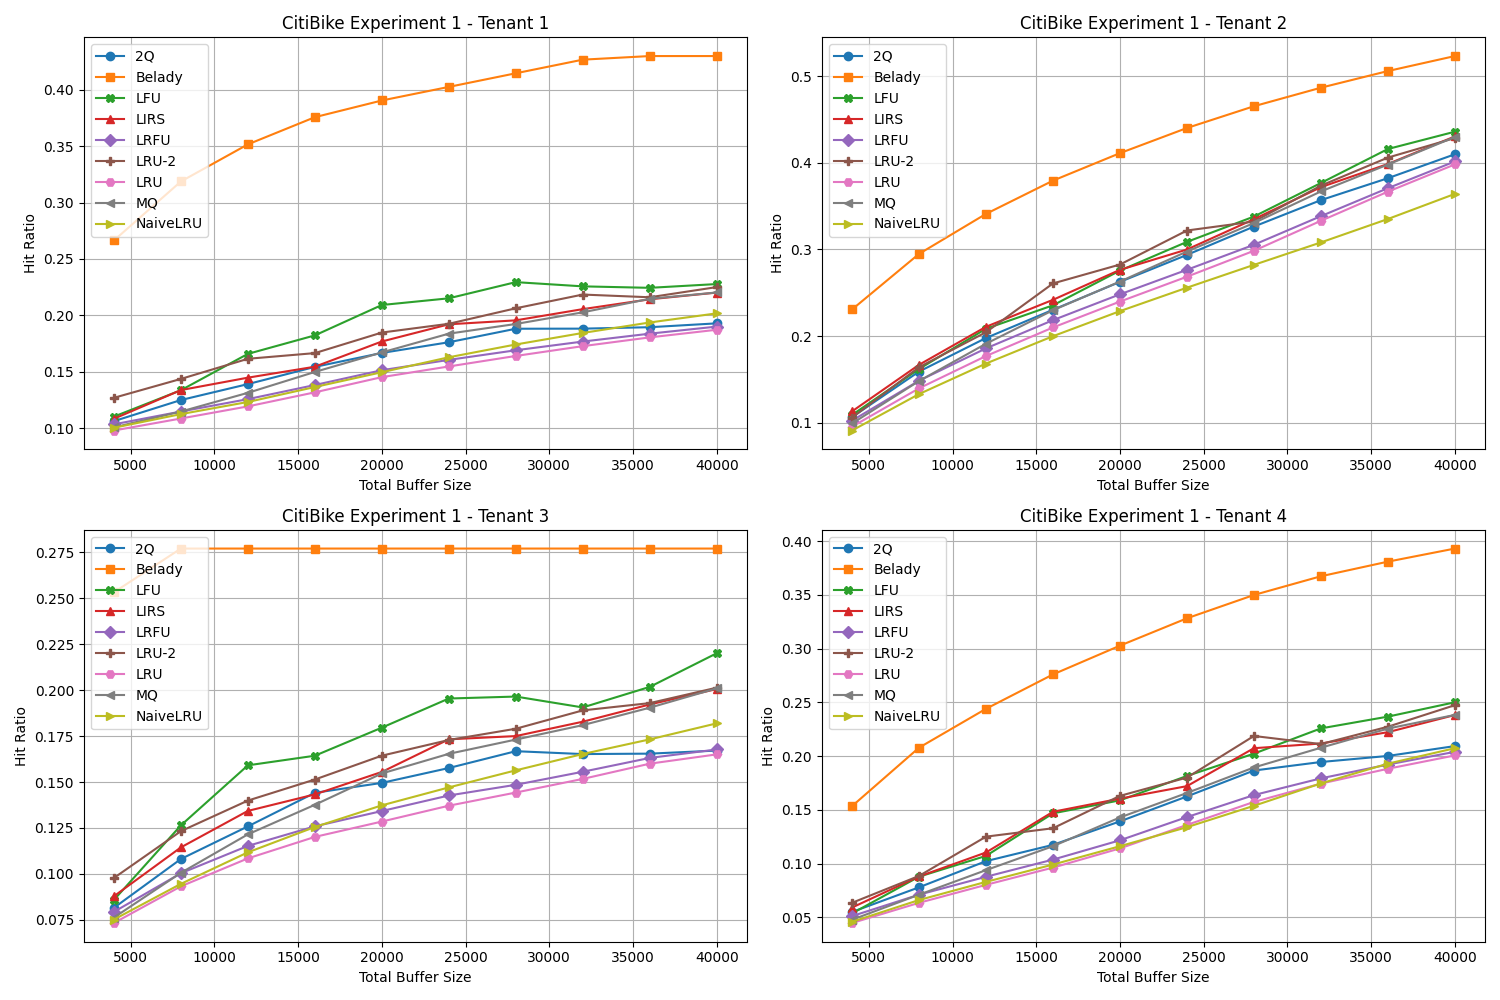
\includegraphics[width=0.75\textwidth]{hit_ratio_per_cache_size_exp_citibike.png}
    \caption{Hit ratio per cache size per tenant for the CitiBike dataset (first experiment)}
    \label{fig:hit_ratio_per_cache_size_exp_citibike}
\end{figure}

\newpage

\begin{table}[ht]
    \centering
    \small
    \caption{Penalty function score (fault score) per cache size for the CitiBike dataset (first experiment)}
    \csvautotabular{data/fault_score_per_buffer_size_citibike_1.csv}
    \label{tab:fault-score-per-buffer-size-citibike}
\end{table}

\begin{table}[ht]
    \centering
    \small
    \caption{Penalty function score (fault score) per cache size for the CitiBike dataset (second experiment)}
    \csvautotabular{data/fault_score_per_buffer_size_citibike_2.csv}
    \label{tab:fault-score-per-buffer-size-citibike-2}
\end{table}

\begin{table}[ht]
    \centering
    \small
    \caption{Penalty function score (fault score) per cache size for the CitiBike dataset (third experiment)}
    \csvautotabular{data/fault_score_per_buffer_size_citibike_3.csv}
    \label{tab:fault-score-per-buffer-size-citibike-3}
\end{table}

\subsection{Fault Score Experiment}

In the fault score experiment, we ran the cache eviction policies in the BrightKite experiment 
and in the three CitiBike experiments, and computed the penalty function score (fault score) 
for each cache eviction policy in each experiment.

The cache size recommendations for each tenant were set as described in the dataset processing 
section.

Minimum buffer sizes, maximum buffer sizes, and total buffer size were set as described in 
the experiments overview section.

Tenant priorities were set depending on the number of accesses of each tenant and the number of
unique items of each tenant.

\subsubsection*{Results}

The penalty function score (fault score) per dataset on the Fault Score Experiment is shown in
Table \ref{tab:fault-score-per-experiment-dataset}.

We observe that LRU solution outperforms NaiveLRU solution for all datasets in the penalty 
function score (fault score) metric, showcasing the positive impact of the Fault Ratio with
Cache Used Policy.

LIRS, LRU-2 and MQ solutions perform particularly well in general accross all datasets.

Overall the results are very good, showcasing that it is possible to achieve a low fault score
with the proposed solution achieving similar results to the baseline solution with a 20\% higher
cache size.

\begin{table}[H]
  \centering
  \small
  \caption{Penalty function score (fault score) per dataset}
  \csvautotabular{data/fault_score_per_solution_per_experiment.csv}
  \label{tab:fault-score-per-experiment-dataset}
\end{table}